%%%%%%%% ICML 2019 EXAMPLE LATEX SUBMISSION FILE %%%%%%%%%%%%%%%%%

\documentclass{article}

% Recommended, but optional, packages for figures and better typesetting:
\usepackage{microtype}
\usepackage{graphicx}
\usepackage{amssymb}
\usepackage{amsmath}
\usepackage{lipsum}
\usepackage{subfigure}
\usepackage{booktabs} % for professional tables
\usepackage[utf8]{inputenc}
\usepackage{cite}
%Includes "References" in the table of contents
\usepackage[nottoc]{tocbibind}

% hyperref makes hyperlinks in the resulting PDF.
% If your build breaks (sometimes temporarily if a hyperlink spans a page)
% please comment out the following usepackage line and replace
% \usepackage{icml2019} with \usepackage[nohyperref]{icml2019} above.
\usepackage{hyperref}

% Attempt to make hyperref and algorithmic work together better:
\newcommand{\theHalgorithm}{\arabic{algorithm}}

% Use the following line for the initial blind version submitted for review:
%\usepackage{icml2019}

% If accepted, instead use the following line for the camera-ready submission:
\usepackage[accepted]{icml2019}

% The \icmltitle you define below is probably too long as a header.
% Therefore, a short form for the running title is supplied here:
\icmltitlerunning{An Exploration of Universal Adversarial Perturbation in Deep Learning}

\begin{document}

\twocolumn[
\icmltitle{An Exploration of Universal Adversarial Perturbation in Deep Learning}

% It is OKAY to include author information, even for blind
% submissions: the style file will automatically remove it for you
% unless you've provided the [accepted] option to the icml2019
% package.

% List of affiliations: The first argument should be a (short)
% identifier you will use later to specify author affiliations
% Academic affiliations should list Department, University, City, Region, Country
% Industry affiliations should list Company, City, Region, Country

% You can specify symbols, otherwise they are numbered in order.
% Ideally, you should not use this facility. Affiliations will be numbered
% in order of appearance and this is the preferred way.
\icmlsetsymbol{equal}{*}

\begin{icmlauthorlist}
\icmlauthor{Yuan Gao}{}
\icmlauthor{Lingfeng Zhang}{}
\icmlauthor{Hongfan Mu}{}
\icmlauthor{Wei Li}{}
\icmlauthor{Peng Yu}{}
\end{icmlauthorlist}

% You may provide any keywords that you
% find helpful for describing your paper; these are used to populate
% the "keywords" metadata in the PDF but will not be shown in the document
\icmlkeywords{Machine Learning, ICML}

\vskip 0.3in
]

% this must go after the closing bracket ] following \twocolumn[ ...

% This command actually creates the footnote in the first column
% listing the affiliations and the copyright notice.
% The command takes one argument, which is text to display at the start of the footnote.
% The \icmlEqualContribution command is standard text for equal contribution.
% Remove it (just {}) if you do not need this facility.

%\printAffiliationsAndNotice{}  % leave blank if no need to mention equal contribution
% \printAffiliationsAndNotice{\icmlEqualContribution} % otherwise use the standard text.

\begin{abstract}
Given a state-of-art deep neural network classifier, we realize the existence of a universal(image-agnostic) and very small perturbation vector that causes natural images to be misclassified with high probability. Under this circumstance, the conditions of generating universal adversarial perturbation have been investigated:
\begin{itemize}
    \item The existence of universal adversarial perturbation under different data complexity
    \item The existence of universal adversarial perturbation under different classifier model complexity
\end{itemize}
The goal of project is to find whether there exit relations among data complexity, classifier model complexity, and universal adversarial perturbation.
\end{abstract}

\section{Introduction}
With the rapid development of deep learning, it has shown its excellent performance in image classification, object recognition, image processing, natural language processing, etc. Deep learning has helped us solve many complex problems, such as the Go problem. The complexity of Go's game tree reached 10\textsuperscript{300}, and no one thought that the machine could completely crack it before Alphago came out. Alphago defeated Lee Sedol, Jie Ke and other masters one after another, showing its powerful strength.

Compared with traditional machine learning algorithms, deep learning has advantages in many aspects. First of all, deep learning does not require a lot of feature processing on the input data. Processing input data features is a very difficult task and requires extensive expert knowledge. This means that models designed using machine learning algorithms tend to focus on a specific field and have poor transferability. It is impossible to use the model used to analyze problems in the financial field to deal with problems in other fields. However, for deep learning, we do not need to perform feature processing on the input data. We can directly input the data into the deep learning model, and the model will learn the features of the data on its own. This allow the model to have some transferability. Secondly, deep learning is easier to improve the accuracy of the model compared to traditional machine learning algorithms. Sometimes increasing the amount of input data can improve the accuracy of deep learning models.However this is unrealistic for machine learning algorithms.

Because of these characteristics, deep learning is widely used in our daily lives. Face recognition unlocked first by Apple has become standard on today's phones. Voice assistants like Siri, Alexa, and Google Assistant have also gradually become an integral part of our lives. Unmanned driving will also become mainstream in the near future. Tesla's Autopilot has been made available on highways and will soon be available on urban roads.

When deep learning is widely used in life, its safety issues have gradually been paid attention to by people. No system can be said to be 100\%\ safe, and deep learning models are no exception. ~\cite{Szegedy42503}  proposed an attack on deep learning-based image classification models in 2014. They generated small perturbations on the images and input changed images into state-of-art deep neural networks. The results showed that most of these pictures were misclassified with high probability. This means that small modifications can fool the classifier. This attack on the model is named as \textit{Adversary Attack}

As people continue to study the Adversary attack, ~\cite{Moosavi-Dezfooli_2017_CVPR}  found that a general perturbation can be found in an image-net dataset. Any image in the data set will be misclassified by the classifier after adding this perturbation. They also found that the perturbation produced by their method also has a certain degree of transforbility, it can fool different classifier. This perturbation were named as \textit{Universal adversarial Perturbation}.

Deep learning models are considered as a black box, we know the input data, output data and network architecture. And we also know it will bring good performance. However, we are difficult to know why its performance is so good. Taking image classification as an example, we cannot intuitively understand the classification criteria of deep learning models. This is also the reason why it is difficult to find the conditions for generating universal adversarial perturbation. 

Adversarial perturbation makes errors in deep learning models that perform well. This will cause serious security threats to applications based on deep learning that have been applied to life. In 2017, ~\cite{Kurakin45818} proposed that adversarial perturbation can be deployed in the physical world. As a simple example, if someone adds an adversarial perturbation to a stop sign, autonomous vehicles will have a high probability of misidentifying the stop sign and cause a traffic accident. Universal adversarial perturbation makes it easier to apply attacks to different scenarios without the need to customize perturbation examples for each scenario. So we want to do research on universal adversarial perturbation.

In this report, we investigate and study the conditions for generating universal adversarial perturbation, and look for the existence of universal adversarial perturbation under different data complexity, classifier model complexity and other relative parameters.And explore the relationship between these parameters and universal adversarial perturbation.

The remaining of the report is organized as fellow. Section 2 introduces the related works of the adversarial perturbation. Section 3 introduces the methods for generating adversarial perturbation. We use the method introduced in Section 3 to generate universal adversarial perturbation under different parameters in Section 4 and analyze results in Section 5. In Section 6 we discuss and analyze the problems found in the experiment and make simple plans for future work. Finally in section VII we try to draw simple conclusions based on our experimental results.  

% \begin{center}
% \textbf{\texttt{http://icml.cc/}}
% \end{center}

% \begin{itemize}
% \item Submissions must be in PDF\@.
% \item Submitted papers can be up to eight pages long, not including references, and up to twelve pages when references and acknowledgments are included. Any paper exceeding this length will automatically be rejected. 
% \item \textbf{Do not include author information or acknowledgements} in your
%     initial submission.
% \item Your paper should be in \textbf{10 point Times font}.
% \item Make sure your PDF file only uses Type-1 fonts.
% \item Place figure captions \emph{under} the figure (and omit titles from inside
%     the graphic file itself). Place table captions \emph{over} the table.
% \item References must include page numbers whenever possible and be as complete
%     as possible. Place multiple citations in chronological order.
% \item Do not alter the style template; in particular, do not compress the paper
%     format by reducing the vertical spaces.
% \item Keep your abstract brief and self-contained, one paragraph and roughly
%     4--6 sentences. Gross violations will require correction at the
%     camera-ready phase. The title should have content words capitalized.
% \end{itemize}

% \subsection{Submitting Papers}

% \textbf{Paper Deadline:} The deadline for paper submission that is
% advertised on the conference website is strict. If your full,
% anonymized, submission does not reach us on time, it will not be
% considered for publication. 

% \textbf{Anonymous Submission:} ICML uses double-blind review: no identifying
% author information may appear on the title page or in the paper
% itself. Section~\ref{author info} gives further details.

% \textbf{Simultaneous Submission:} ICML will not accept any paper which,
% at the time of submission, is under review for another conference or
% has already been published. This policy also applies to papers that
% overlap substantially in technical content with conference papers
% under review or previously published. ICML submissions must not be
% submitted to other conferences during ICML's review period. Authors
% may submit to ICML substantially different versions of journal papers
% that are currently under review by the journal, but not yet accepted
% at the time of submission. Informal publications, such as technical
% reports or papers in workshop proceedings which do not appear in
% print, do not fall under these restrictions.

% \medskip

% Authors must provide their manuscripts in \textbf{PDF} format.
% Furthermore, please make sure that files contain only embedded Type-1 fonts
% (e.g.,~using the program \texttt{pdffonts} in linux or using
% File/DocumentProperties/Fonts in Acrobat). Other fonts (like Type-3)
% might come from graphics files imported into the document.

% Authors using \textbf{Word} must convert their document to PDF\@. Most
% of the latest versions of Word have the facility to do this
% automatically. Submissions will not be accepted in Word format or any
% format other than PDF\@. Really. We're not joking. Don't send Word.

% Those who use \textbf{\LaTeX} should avoid including Type-3 fonts.
% Those using \texttt{latex} and \texttt{dvips} may need the following
% two commands:

% {\footnotesize
% \begin{verbatim}
% dvips -Ppdf -tletter -G0 -o paper.ps paper.dvi
% ps2pdf paper.ps
% \end{verbatim}}
% It is a zero following the ``-G'', which tells dvips to use
% the config.pdf file. Newer \TeX\ distributions don't always need this
% option.

% Using \texttt{pdflatex} rather than \texttt{latex}, often gives better
% results. This program avoids the Type-3 font problem, and supports more
% advanced features in the \texttt{microtype} package.

% \textbf{Graphics files} should be a reasonable size, and included from
% an appropriate format. Use vector formats (.eps/.pdf) for plots,
% lossless bitmap formats (.png) for raster graphics with sharp lines, and
% jpeg for photo-like images.

% The style file uses the \texttt{hyperref} package to make clickable
% links in documents. If this causes problems for you, add
% \texttt{nohyperref} as one of the options to the \texttt{icml2019}
% usepackage statement.


% \subsection{Submitting Final Camera-Ready Copy}

% The final versions of papers accepted for publication should follow the
% same format and naming convention as initial submissions, except that
% author information (names and affiliations) should be given. See
% Section~\ref{final author} for formatting instructions.

% The footnote, ``Preliminary work. Under review by the International
% Conference on Machine Learning (ICML). Do not distribute.'' must be
% modified to ``\textit{Proceedings of the
% $\mathit{36}^{th}$ International Conference on Machine Learning},
% Long Beach, USA, 2019.
% Copyright 2019 by the author(s).''

% For those using the \textbf{\LaTeX} style file, this change (and others) is
% handled automatically by simply changing
% $\mathtt{\backslash usepackage\{icml2019\}}$ to
% $$\mathtt{\backslash usepackage[accepted]\{icml2019\}}$$
% Authors using \textbf{Word} must edit the
% footnote on the first page of the document themselves.

% Camera-ready copies should have the title of the paper as running head
% on each page except the first one. The running title consists of a
% single line centered above a horizontal rule which is $1$~point thick.
% The running head should be centered, bold and in $9$~point type. The
% rule should be $10$~points above the main text. For those using the
% \textbf{\LaTeX} style file, the original title is automatically set as running
% head using the \texttt{fancyhdr} package which is included in the ICML
% 2019 style file package. In case that the original title exceeds the
% size restrictions, a shorter form can be supplied by using

% \verb|\icmltitlerunning{...}|

% just before $\mathtt{\backslash begin\{document\}}$.
% Authors using \textbf{Word} must edit the header of the document themselves.

\section{Related work} 
\subsection{Notation}
\textit{x}, original images that do not be modified from the dataset.
\texttit{$x'$}, the adversarial images which are modified from the dataset. What should be noticed is that the adversarial images will not be misclassified sometimes.
\texttit{l}, the label of class in the classification problem.
\texttit{$l'$}, the label of class in the adversarial class.
\texttit{$\eta$}, the size of the adversarial perturbation. Goodfellow et al. \cite{goodfellow2014explaining} proposed that, in most cases, the $L_\infty$ of the perturbation should be less than $\eta$. $\eta$ is also specified as pixel values in the range [0,255]. Based on the research from Szegedy et al. \cite{Szegedy42503}, 2014, there are also some work focus on minimizing the size of the perturbation directly instead of importing a constrain on the size of the perturbation.
\texttit{$J_f(x,l)$} represents the cost function of \tettit{f}. \subsection{Generating adversarial examples}
 In this subsection, multiple methods that are used to generate adversarial examples will be discussed.
\begin{enumerate}
\item L-BFGS Attack \\
The adversarial examples attacks against deep neural networks is first introduced by Szegedy et al.\cite{Szegedy42503} in 2014. L-BFGS, which aims to find an appropriate constant \texttit{c}, is used to solve the general targeted misclassified problem:
$$\underset{x'}{min}\;\;c{\| \eta \|+ J_\theta(x',l')} $$ $$s.t.\;\; x' \in[0,1],$$
where $ l′ $ denotes the output label of $ x′ $.
\item Fast Gradient Sign Method(FGSM)\\
L-BFGS is a typical linear-searching method requires large time consuming. In 2014, Goodfellow et al.\cite{goodfellow2014explaining} proposed a more computationally efficient method named Fast Gradient Sign Method, updating gradient at each pixel within one step. The perturbation is:
$$\eta = \epsilon sign(\bigtriangledown_x{J_\theta(x,l)}),$$
which can be generated by computing back-propagation.
FGSM is a much more simple way to generate adversarial examples:$$x' = x + \eta,$$
where $\epsilon$ can be selected ranged [0,1] that represents the magnitude of the perturbation. Since the deep neural network in high dimension shows that it can not defence adversarial examples, Fast Gradient Value method, which was proposed by \cite{Rozsa}. The sign of the gradient was replaced by the raw gradient in this method that is different from previous work:
$$\eta = \bigtriangledown_xJ(\theta,x,l).$$
\item Jacobian-based Saliency Map Attack (JSMA) \\
Jacobian-based Saliency Map Attack was first proposed by Papernot et al. \cite{JSMA}which computes Jacobian matrix of input x :
$$J_{F(x)} = \frac{\partial F(x)}{\partial x} = [\frac{\partial F_j(x)}{\partial x_i}]_{i \times j}$$
F represents the second-to-last layer, while Carlini and Wagner \cite{Carlini} tends to replace it with the output of the softmax layer, from which, they observe that the most essential modification to the output was contributed by the input features of \texttit{x}. What was found as well is that a small perturbation on features can lead to the misclassification of neural network with inducing the large output changes.\\
Because of the observation founded, two adversarial salience maps were created to select the features in each iteration, which contributes to improving the success of misclassifying adversarial examples by modifying a slight changes on input images.

\item C&W’s Attack \\
Carlini and Wagner defined a new objective function \texttit{g} that is different from previous work \cite{Carlini_and_Wagner}\cite{Magnet}: $$\underset{\eta}{min}\;\; \|\eta\|_p+c \cdot g(\eta + x) $$
$$s.t.\;\; x+ \eta \in[0,1]^n,$$
where $g(x) \ge 0$ if and only if $f(x)=l$. From their research\cite{Carlini_and_Wagner}\cite{Magnet}, C\&W’s Attack is effective for most of existing adversarial detecting defenses. In this method, seven different objective functions were proposed.
In their research, the constant \texttit{c} will not be found in the gradient search, and the optimal result will not be obtained if the gradients of $\| \eta \| _p$ and $g(x + \eta)$ are not in the same scale.
\item One Pixel Attack \\
Adversarial examples can be generated by modifying on just one pixel in images, which is called one pixel attack\cite{Su}. The problem of finding one pixel adversarial examples can be defined as:
$$\underset{x'}{min} \;\; J(f(x'),l')$$
$$s.t. \;\; \|\eta\|_0 \leq \epsilon_0, $$
where $\epsilon_0$ = 1 is defined to modify only one pixel.
\end{enumerate}
\subsection{Adversarial examples in an image classification task}
The original images will be trained by an established image classifier to obtain the correct class labels of each. Adversarial images are then modified through the original images with small perturbations that can not be recognized by human. These small perturbations will lead to the miss-classification and the miss-classified label will be obtained from the classier at the same time.
Here, in our experiment, the original images are all generated by generating models which are based on deep learning architectures with different number of convectional layers and fully connected layers according to different data complexity.


% \subsection{Length and Dimensions}

% Submitted papers can be up to eight pages long, not including references, and up to twelve pages when references and acknowledgments are included.
% Acknowledgements should be limited to grants and people who contributed to the paper.
% Any submission that exceeds
% this page limit, or that diverges significantly from the specified format,
% will be rejected without review.

% The text of the paper should be formatted in two columns, with an
% overall width of 6.75~inches, height of 9.0~inches, and 0.25~inches
% between the columns. The left margin should be 0.75~inches and the top
% margin 1.0~inch (2.54~cm). The right and bottom margins will depend on
% whether you print on US letter or A4 paper, but all final versions
% must be produced for US letter size.

% The paper body should be set in 10~point type with a vertical spacing
% of 11~points. Please use Times typeface throughout the text.

% \subsection{Title}

% The paper title should be set in 14~point bold type and centered
% between two horizontal rules that are 1~point thick, with 1.0~inch
% between the top rule and the top edge of the page. Capitalize the
% first letter of content words and put the rest of the title in lower
% case.

% \subsection{Author Information for Submission}
% \label{author info}

% ICML uses double-blind review, so author information must not appear. If
% you are using \LaTeX\/ and the \texttt{icml2019.sty} file, use
% \verb+\icmlauthor{...}+ to specify authors and \verb+\icmlaffiliation{...}+ to specify affiliations. (Read the TeX code used to produce this document for an example usage.) The author information
% will not be printed unless \texttt{accepted} is passed as an argument to the
% style file.
% Submissions that include the author information will not
% be reviewed.

% \subsubsection{Self-Citations}

% If you are citing published papers for which you are an author, refer
% to yourself in the third person. In particular, do not use phrases
% that reveal your identity (e.g., ``in previous work \cite{langley00}, we
% have shown \ldots'').

% Do not anonymize citations in the reference section. The only exception are manuscripts that are
% not yet published (e.g., under submission). If you choose to refer to
% such unpublished manuscripts \cite{anonymous}, anonymized copies have
% to be submitted
% as Supplementary Material via CMT\@. However, keep in mind that an ICML
% paper should be self contained and should contain sufficient detail
% for the reviewers to evaluate the work. In particular, reviewers are
% not required to look at the Supplementary Material when writing their
% review.

% \subsubsection{Camera-Ready Author Information}
% \label{final author}

% If a paper is accepted, a final camera-ready copy must be prepared.
% %
% For camera-ready papers, author information should start 0.3~inches below the
% bottom rule surrounding the title. The authors' names should appear in 10~point
% bold type, in a row, separated by white space, and centered. Author names should
% not be broken across lines. Unbolded superscripted numbers, starting 1, should
% be used to refer to affiliations.

% Affiliations should be numbered in the order of appearance. A single footnote
% block of text should be used to list all the affiliations. (Academic
% affiliations should list Department, University, City, State/Region, Country.
% Similarly for industrial affiliations.)

% Each distinct affiliations should be listed once. If an author has multiple
% affiliations, multiple superscripts should be placed after the name, separated
% by thin spaces. If the authors would like to highlight equal contribution by
% multiple first authors, those authors should have an asterisk placed after their
% name in superscript, and the term ``\textsuperscript{*}Equal contribution"
% should be placed in the footnote block ahead of the list of affiliations. A
% list of corresponding authors and their emails (in the format Full Name
% \textless{}email@domain.com\textgreater{}) can follow the list of affiliations.
% Ideally only one or two names should be listed.

% A sample file with author names is included in the ICML2019 style file
% package. Turn on the \texttt{[accepted]} option to the stylefile to
% see the names rendered. All of the guidelines above are implemented
% by the \LaTeX\ style file.

% \subsection{Abstract}

% The paper abstract should begin in the left column, 0.4~inches below the final
% address. The heading `Abstract' should be centered, bold, and in 11~point type.
% The abstract body should use 10~point type, with a vertical spacing of
% 11~points, and should be indented 0.25~inches more than normal on left-hand and
% right-hand margins. Insert 0.4~inches of blank space after the body. Keep your
% abstract brief and self-contained, limiting it to one paragraph and roughly 4--6
% sentences. Gross violations will require correction at the camera-ready phase.

% \subsection{Partitioning the Text}

% You should organize your paper into sections and paragraphs to help
% readers place a structure on the material and understand its
% contributions.

% \subsubsection{Sections and Subsections}

% Section headings should be numbered, flush left, and set in 11~pt bold
% type with the content words capitalized. Leave 0.25~inches of space
% before the heading and 0.15~inches after the heading.

% Similarly, subsection headings should be numbered, flush left, and set
% in 10~pt bold type with the content words capitalized. Leave
% 0.2~inches of space before the heading and 0.13~inches afterward.

% Finally, subsubsection headings should be numbered, flush left, and
% set in 10~pt small caps with the content words capitalized. Leave
% 0.18~inches of space before the heading and 0.1~inches after the
% heading.

% Please use no more than three levels of headings.

% \subsubsection{Paragraphs and Footnotes}

% Within each section or subsection, you should further partition the
% paper into paragraphs. Do not indent the first line of a given
% paragraph, but insert a blank line between succeeding ones.

% You can use footnotes\footnote{Footnotes
% should be complete sentences.} to provide readers with additional
% information about a topic without interrupting the flow of the paper.
% Indicate footnotes with a number in the text where the point is most
% relevant. Place the footnote in 9~point type at the bottom of the
% column in which it appears. Precede the first footnote in a column
% with a horizontal rule of 0.8~inches.\footnote{Multiple footnotes can
% appear in each column, in the same order as they appear in the text,
% but spread them across columns and pages if possible.}

% \begin{figure}[ht]
% \vskip 0.2in
% \begin{center}
% \centerline{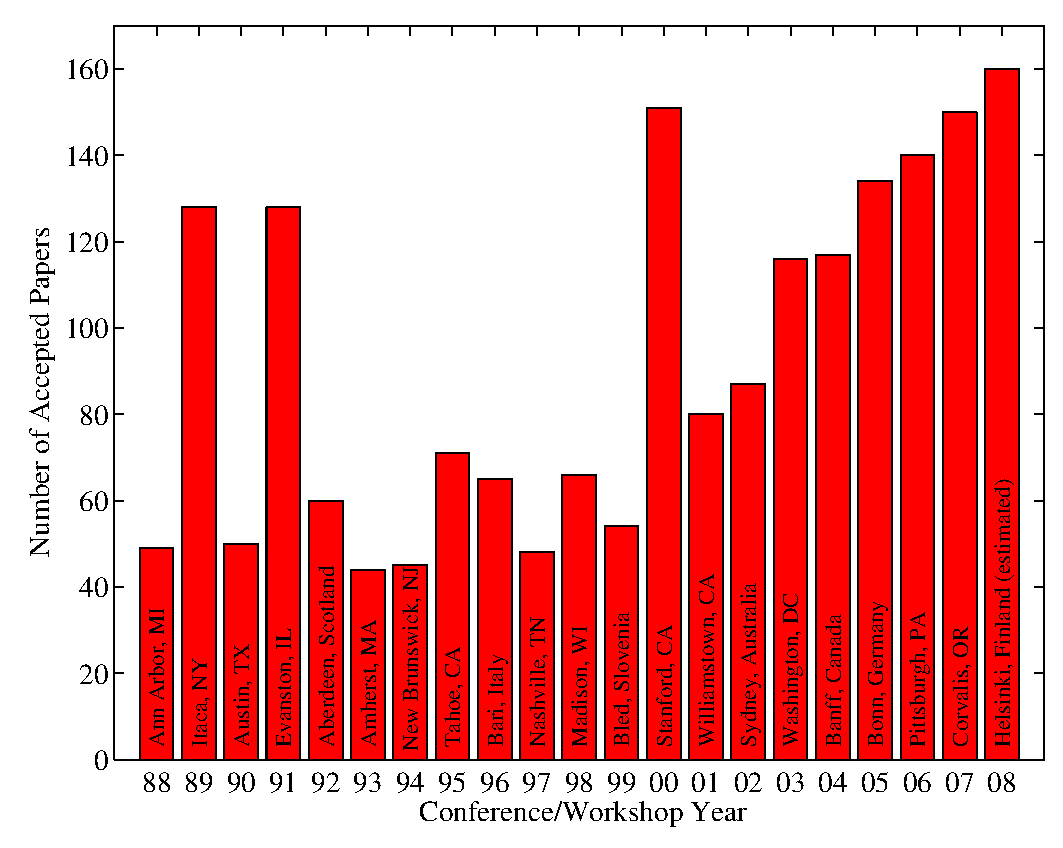
\includegraphics[width=\columnwidth]{icml_numpapers}}
% \caption{Historical locations and number of accepted papers for International
% Machine Learning Conferences (ICML 1993 -- ICML 2008) and International
% Workshops on Machine Learning (ML 1988 -- ML 1992). At the time this figure was
% produced, the number of accepted papers for ICML 2008 was unknown and instead
% estimated.}
% \label{icml-historical}
% \end{center}
% \vskip -0.2in
% \end{figure}

% \subsection{Figures}

% You may want to include figures in the paper to illustrate
% your approach and results. Such artwork should be centered,
% legible, and separated from the text. Lines should be dark and at
% least 0.5~points thick for purposes of reproduction, and text should
% not appear on a gray background.

% Label all distinct components of each figure. If the figure takes the
% form of a graph, then give a name for each axis and include a legend
% that briefly describes each curve. Do not include a title inside the
% figure; instead, the caption should serve this function.

% Number figures sequentially, placing the figure number and caption
% \emph{after} the graphics, with at least 0.1~inches of space before
% the caption and 0.1~inches after it, as in
% Figure~\ref{icml-historical}. The figure caption should be set in
% 9~point type and centered unless it runs two or more lines, in which
% case it should be flush left. You may float figures to the top or
% bottom of a column, and you may set wide figures across both columns
% (use the environment \texttt{figure*} in \LaTeX). Always place
% two-column figures at the top or bottom of the page.

% \subsection{Algorithms}

% If you are using \LaTeX, please use the ``algorithm'' and ``algorithmic''
% environments to format pseudocode. These require
% the corresponding stylefiles, algorithm.sty and
% algorithmic.sty, which are supplied with this package.
% Algorithm~\ref{alg:example} shows an example.

% \begin{algorithm}[tb]
%   \caption{Bubble Sort}
%   \label{alg:example}
% \begin{algorithmic}
%   \STATE {\bfseries Input:} data $x_i$, size $m$
%   \REPEAT
%   \STATE Initialize $noChange = true$.
%   \FOR{$i=1$ {\bfseries to} $m-1$}
%   \IF{$x_i > x_{i+1}$}
%   \STATE Swap $x_i$ and $x_{i+1}$
%   \STATE $noChange = false$
%   \ENDIF
%   \ENDFOR
%   \UNTIL{$noChange$ is $true$}
% \end{algorithmic}
% \end{algorithm}

% \subsection{Tables}

% You may also want to include tables that summarize material. Like
% figures, these should be centered, legible, and numbered consecutively.
% However, place the title \emph{above} the table with at least
% 0.1~inches of space before the title and the same after it, as in
% Table~\ref{sample-table}. The table title should be set in 9~point
% type and centered unless it runs two or more lines, in which case it
% should be flush left.

% % Note use of \abovespace and \belowspace to get reasonable spacing
% % above and below tabular lines.

% \begin{table}[t]
% \caption{Classification accuracies for naive Bayes and flexible
% Bayes on various data sets.}
% \label{sample-table}
% \vskip 0.15in
% \begin{center}
% \begin{small}
% \begin{sc}
% \begin{tabular}{lcccr}
% \toprule
% Data set & Naive & Flexible & Better? \\
% \midrule
% Breast    & 95.9$\pm$ 0.2& 96.7$\pm$ 0.2& $\surd$ \\
% Cleveland & 83.3$\pm$ 0.6& 80.0$\pm$ 0.6& $\times$\\
% Glass2    & 61.9$\pm$ 1.4& 83.8$\pm$ 0.7& $\surd$ \\
% Credit    & 74.8$\pm$ 0.5& 78.3$\pm$ 0.6&         \\
% Horse     & 73.3$\pm$ 0.9& 69.7$\pm$ 1.0& $\times$\\
% Meta      & 67.1$\pm$ 0.6& 76.5$\pm$ 0.5& $\surd$ \\
% Pima      & 75.1$\pm$ 0.6& 73.9$\pm$ 0.5&         \\
% Vehicle   & 44.9$\pm$ 0.6& 61.5$\pm$ 0.4& $\surd$ \\
% \bottomrule
% \end{tabular}
% \end{sc}
% \end{small}
% \end{center}
% \vskip -0.1in
% \end{table}

% Tables contain textual material, whereas figures contain graphical material.
% Specify the contents of each row and column in the table's topmost
% row. Again, you may float tables to a column's top or bottom, and set
% wide tables across both columns. Place two-column tables at the
% top or bottom of the page.

% \subsection{Citations and References}

% Please use APA reference format regardless of your formatter
% or word processor. If you rely on the \LaTeX\/ bibliographic
% facility, use \texttt{natbib.sty} and \texttt{icml2019.bst}
% included in the style-file package to obtain this format.

% Citations within the text should include the authors' last names and
% year. If the authors' names are included in the sentence, place only
% the year in parentheses, for example when referencing Arthur Samuel's
% pioneering work \yrcite{Samuel59}. Otherwise place the entire
% reference in parentheses with the authors and year separated by a
% comma \cite{Samuel59}. List multiple references separated by
% semicolons \cite{kearns89,Samuel59,mitchell80}. Use the `et~al.'
% construct only for citations with three or more authors or after
% listing all authors to a publication in an earlier reference \cite{MachineLearningI}.

% Authors should cite their own work in the third person
% in the initial version of their paper submitted for blind review.
% Please refer to Section~\ref{author info} for detailed instructions on how to
% cite your own papers.

% Use an unnumbered first-level section heading for the references, and use a
% hanging indent style, with the first line of the reference flush against the
% left margin and subsequent lines indented by 10 points. The references at the
% end of this document give examples for journal articles \cite{Samuel59},
% conference publications \cite{langley00}, book chapters \cite{Newell81}, books
% \cite{DudaHart2nd}, edited volumes \cite{MachineLearningI}, technical reports
% \cite{mitchell80}, and dissertations \cite{kearns89}.

% Alphabetize references by the surnames of the first authors, with
% single author entries preceding multiple author entries. Order
% references for the same authors by year of publication, with the
% earliest first. Make sure that each reference includes all relevant
% information (e.g., page numbers).

% Please put some effort into making references complete, presentable, and
% consistent. If using bibtex, please protect capital letters of names and
% abbreviations in titles, for example, use \{B\}ayesian or \{L\}ipschitz
% in your .bib file.

% \subsection{Software and Data}

% We strongly encourage the publication of software and data with the
% camera-ready version of the paper whenever appropriate. This can be
% done by including a URL in the camera-ready copy. However, do not
% include URLs that reveal your institution or identity in your
% submission for review. Instead, provide an anonymous URL or upload
% the material as ``Supplementary Material'' into the CMT reviewing
% system. Note that reviewers are not required to look at this material
% when writing their review.

% % Acknowledgements should only appear in the accepted version.

\section{Method For Generating Universal Adversarial Examples }
\noindent In the experiment, Universal adversarial perturbations algorithm ~\cite{Moosavi-Dezfooli_2017_CVPR} was used to find the universal attack, and in the algorithm, DeepFool ~\cite{Moosavi-Dezfooli_2016_CVPR} is another method that we used to find perturbations for individual data point and to update the universal attack.

\subsection{DeepFool}
DeepFool is a non-targeted attack method, i.e. its objective is only to fool a classifier to a different class. In DeepFool, minimal adversarial perturbation is defined as the closest distance from the target data point to the correspondent decision boundary (a hyperplane) the attacker want to attack. 
\\ \hspace*{\fill} \\Formally, assume a multiclasses classification problem, we have data $x  \in \mathcal{X}$. For each class, there is a hyperplane that separate the feature space where $x$ living in. For a data point $x_0$, it is classified into the class which the small space it lies is separated by those hyperplanes. 
\\ \hspace*{\fill} \\Assume we have a classifier $f$, the minimal perturbation $r$ that make $f(x_0 + r) \neq f(x_0) $ is the one that can send $x_0$ to its nearest decision boundary:
\begin{equation*}
 r = -\frac{f\left(x_{0}\right)}{\|w\|_{2}^{2}} * w \end{equation*}

\noindent Where $w$ is the normal vector of the nearest decision boundary.
 
 
\\ \hspace*{\fill} \\\noindent What the algorithm do is finding the closest hyperplane of $x_0$, pushing it toward the hyperplane and then pushing it a little further, so that $f(x)$ will misclassify $x_0$ as another class.
The following equation gives the equation that calculate the closest hyperplane:
\begin{equation*}
\hat{l}\left(\boldsymbol{x}_{0}\right)=\underset{k \neq \hat{k}\left(\boldsymbol{x}_{0}\right)}{\arg \min } \frac{\left|f_{k}\left(\boldsymbol{x}_{0}\right)-f_{\hat{k}\left(\boldsymbol{x}_{0}\right)}\left(\boldsymbol{x}_{0}\right)\right|}{\left\|\boldsymbol{w}_{k}-\boldsymbol{w}_{\hat{k}\left(\boldsymbol{x}_{0}\right)}\right\|_{2}}
\end{equation*}


\\ \hspace*{\fill} \\\noindent Where $f_{\hat{k}\left(\boldsymbol{x}_{0}\right)}\left(\boldsymbol{x}_{0}\right)$ the classifier’s possibility of the true label of $ x_{0}$, and $f_{k}\left(\boldsymbol{x}_{0}\right)$ is the possibility of the most likely label $k$ that are not equal to $\hat{k}$.
The DeepFool algorithm is given below Figure~\ref{fig:deep_fool_algo}, line 6-10 calculates the closest hyperplane, line 11-12 calculate the minimal perturbation and update $ x_{0}$.

\begin{figure}[h]
    \centering
    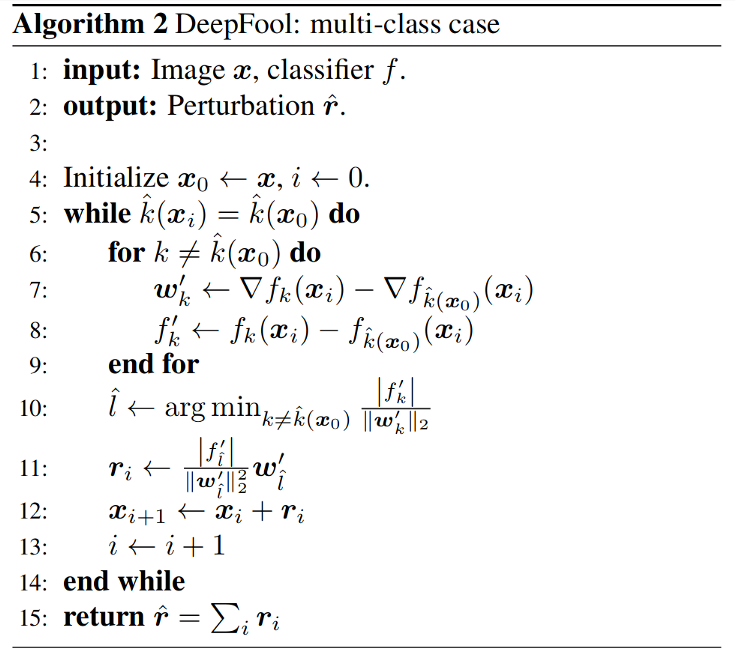
\includegraphics[width=1\linewidth]{deep_fool_algo.png}
    \caption{\small Deep Fool Algorithm}
    \label{fig:deep_fool_algo}
\end{figure}

\subsection{Universal Perturbation}

~\cite{Moosavi-Dezfooli_2017_CVPR} presented the Universal Perturbation method to find a single perturbation that can fool most of the data points in a data set. Assume $\mu$ is the distribution of data $\mathcal{X}$ in $\mathbb{R}^{d}$, and $\hat{k}$ is the classifier that classifier a data point $x \in \mathbb{R}^{d}$ into an estimated label $\hat{k}(x)$, an Universal perturbation $v$ is the one that makes:

\begin{equation*}
\hat{k}(x+v) \neq \hat{k}(x) \mbox{ for most x $\sim \mu$}
\end{equation*}

\noindent There are two constrains to the universal perturbation, firstly, it should be small enough (measured by $\ell_{ \infty}$ norm). secondly, it should be general enough (i.e. to fool ‘most’ data points). So we have:
\begin{equation*}
\|v\|_{p} \leq \xi
\end{equation*}

\begin{equation*}
\underset{x \sim \mu}{\mathbb{P}}(\hat{k}(x+v) \neq \hat{k}(x)) \geq 1-\delta
\end{equation*}
    

\noindent Where $\xi$ controls the magnitude of the perturbation, and $\delta$ controls the percent of data points in the data set that are ‘fooled’.

\\ \hspace*{\fill} \\\noindent The universal perturbation algorithm iterates over data points $x_i  \in \mathcal{X}$ and build up $v$ gradually by calculation the DeepFool perturbation of $x_i $. Concisely, assume that we already have an universal perturbation vector $v$ , for each data point $x_i  \in \mathcal{X}$, as long as $v$ cannot fool $x_i $ on the classifer( $\hat{k}\left(x_{i}+v\right)=\hat{k}\left(x_{i}\right)$), 
	we proceed to calculate the extra minimal DeepFool perturbation $r$ that after being added to the already perturbed $ x_{i} $, the new $ x_{i}+v +r$ can be misclassified. The extra perturbation $r$ is saved as $\Delta v_{i}$ to update $v$.
	\begin{equation*}
	  \Delta v_{i} \leftarrow \arg \min _{r}\left\|r\right\|_{2}  \mbox{  ,  s.t. $\hat{k}\left(x_{i}+v+r\right) \neq \hat{k}\left(x_{i}\right)$}
	\end{equation*}


\noindent The $\Delta v_{i}$ is then constrain into a vector of at most $\ell_{ \infty}$ norm $\xi$ by the following transformation, and the transformed perturbation vector is then used to update the universal perturbation $v$:
\begin{multline*}\label{eq11}
      \mathcal{P}_{p, \xi}\left(v+\Delta v_{i}\right)= \\
  \arg \min _{v^{\prime}}\left\|(v+\Delta v_{i})-v^{\prime}\right\|_{2} \mbox{ ,  s.t. $\left\|v^{\prime}\right\|_{p} \leq \xi$}
\end{multline*}

		\begin{equation*}
				v \leftarrow \mathcal{P}_{p, \xi}\left(v+\Delta v_{i}\right)
			\end{equation*}

\noindent The algorithm iterates over data points in the data set, until the desired “fooling rate” is met. In other word, the algorithm terminates when the rate of misclassification exceeds the threshold $1-\delta$.


\section{Experiment Setup}
In this experiment, relationships between the existence of university perturbation and the dataset complexity, as well as the training model complexity should be found. There are three main steps to process experiments:

\begin{itemize}
    \item Generating images with different complexity levels
    \item Training models with different number of layers
    \item Generating the universal perturbation based on a certain complexity level dataset and a certain number of layers training model. 
\end{itemize}

\subsection{Generating images}

Some assumptions setting: 
\begin{itemize}
    \item images size and channel: 28*28*1
    \item number of classes: 4
    \item images number for each class: 1000
\end{itemize}

Firstly, 4 class baseline images should be created. See Figure~\ref{fig:baseline_image}.To generate these images, setting 1 as the pixel value on separated locations and uniform distribution random number ranged [0,1) on other unfilled locations. Making sure that the training model can recognise different class images. In this case, setting 1 on upper left corner 7*7 pixels and random number on other pixels represents class 0 images. And by the same logic, images of class 1, 2 and 3 are created. 
\begin{figure}[h]
    \centering
    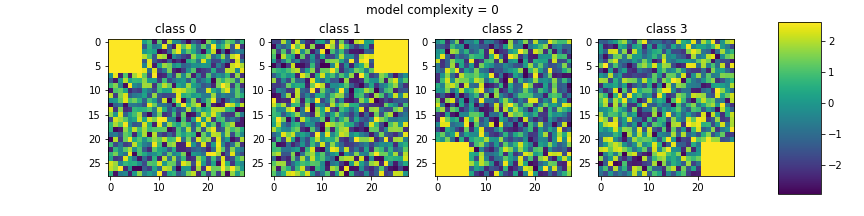
\includegraphics[width=1\linewidth]{demo-0.png}
    \caption{\small 4 class baseline images}
    \label{fig:baseline_image}
\end{figure}

While getting more complex dataset, more convolutional layers in the generating images model(called "images generator") should be added. The relation between them see formula (1). The weights and bias in convolutional layers do not need be learned in the images generator. These parameters are initialized and fixed by random values, uniform distribution random value for weights and normal distribution for bias.

\scriptsize
\begin{equation*}
    number\ of\ layers\ in\ generator\ \propto dataset\ complexity\ level  
\end{equation*}
\normalsize


After 2 layers convolutional computation, the baseline images are transferred into Figure~ \ref{fig:more_complex_image}. These images look like more complex than baseline images intuitively.
\begin{figure}[h]
    \centering
    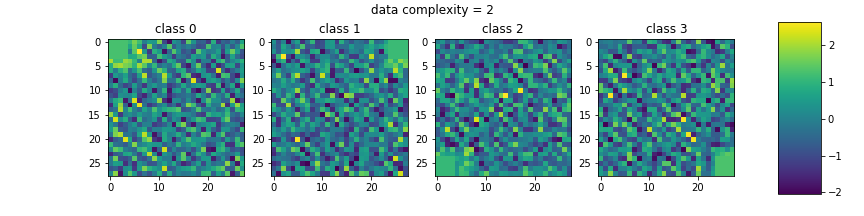
\includegraphics[width=1\linewidth]{demo-2.png}
    \caption{\small 4 class images after 2 convolutional computation}
    \label{fig:more_complex_image}
\end{figure}

It should be mentioned that all pixel values of one image will be close to a certain number(in most cases, close to 0) after original images passing the images generator with many convolutional layers. This is probably because feature boundaries of different class images fades with increasing times of convolutional computations. So, these images pixel values should be scaled. Feature boundary in this experiment is represented by the location of pixels with value 1.

There are several comments and tricks about the images generator model
\begin{itemize}
    
    \item To make sure that adding more layers in the images generator can get more complex dataset, weights in less layers of the images generator should be stored and used again on lower layers of the more layers images generator. Otherwise, if these weights are totally different random values, it will occur that the more layers generator may get lower complex dataset than the less layers generator. This is because all weights of the more layers generator are probably overall smaller than these weights of the less layers generator.
    
    \item This method to generate different complexity level dataset is reasonable because convolutional computation can gradually blur the decision boundary from baseline images dataset with increasing the convolutional layers.
    
    \item The number of convolutional layers in the images generator is in range from 0 to 9. When 10 convolutional layers are used in the generator, training model could not learn the decision boundary of these classes well, meaning testing accuracy is not good enough. This is probably because too many convolutional computations mix up the location information which can be recognised by the training model. In another word, too much layers in images generator will generate "garbage" images which can not be classified by training models well. After 9 layers convolutional computation, the baseline images are transferred into Figure~ \ref{fig:most_complex_image}. It is difficult to recognise which classes these images belong to by human eyes.
    
    \item To compare the size of universal perturbation generated from different complexity level dataset later, these images pixel values should be expanded or shrank to the same scale. So, these images pixels should be normalized after passing these convolutional layers.
    
    \item To avoid too much loss of baseline images' information, the activation function in each convolutional layers in images generator is LeakyRelu because other activation functions like ReLu, sigmoid, tanh or others, may induce values into saturation field, which cause the information loss.
    
    \item In the images generator, only convolutional layers are constructed because pooling layers may lead to the information loss from original images and dense layers may shuffle the location of representative pixels.
\end{itemize}

\begin{figure}[h]
    \centering
    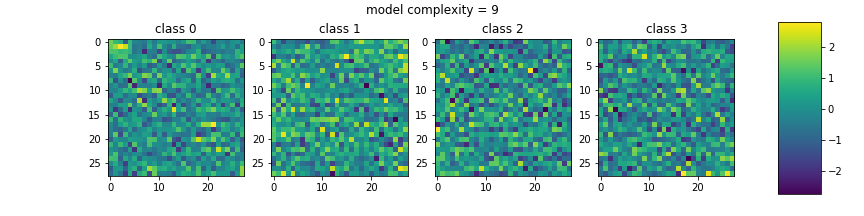
\includegraphics[width=1\linewidth]{demo-9.png}
    \caption{\small 4 class images after 9 convolutional computation}
    \label{fig:most_complex_image}
\end{figure}

The structure of images generator with 4 convolutional layers(dataset complexity level 4) is shown in Table ~\ref{table:generator_structure} and Figure ~\ref{fig:generator_structure}.

\begin{table}
\begin{center}
\begin{tabular}{ |c|c|c|c|c| } 
\hline
Height & Width & Depth & filter Height & filter Width \\
\hline
36 & 36 & 1 & 3 & 3 \\ 
\hline
34 & 34 & 32 & 3 & 3 \\ 
\hline
32 & 32 & 32 & 3 & 3 \\ 
\hline
30 & 30 & 32 & 3 & 3 \\ 
\hline
28 & 28 & 1 & None & None \\ 
\hline
\end{tabular}
\end{center}
\caption{The structure of images generator with 4 convolutional layers}
\label{table:generator_structure}
\end{table}

\begin{figure}[h]
    \centering
    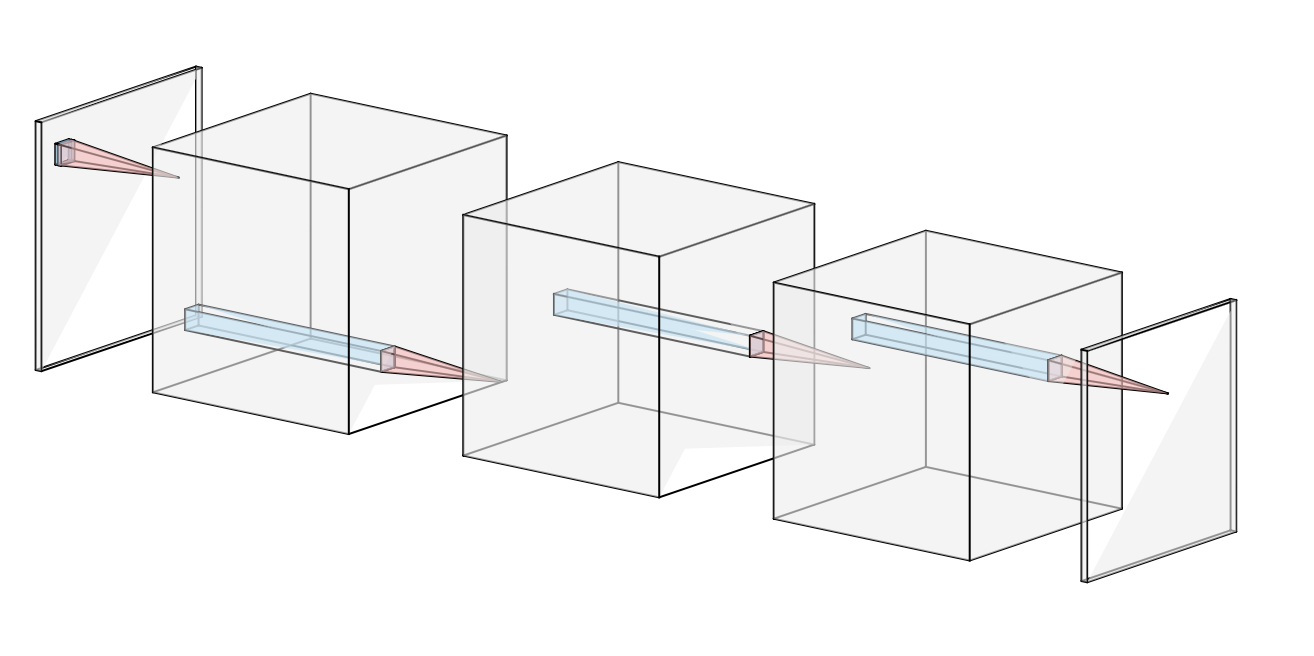
\includegraphics[width=1\linewidth]{generator_structure.png}
    \caption{\small The structure of images generator with 4 convolutional layers}
    \label{fig:generator_structure}
\end{figure}

To find the relation between the dataset complexity and the universal perturbation, the number of training model layers should be fixed on 4.
\subsection{Training models}

To get different complex training models, adding different number of layers can achieve this goal. Seven kinds of layers number are record: 3, 5, 8, 11, 14, 17 and 20. 3 layers training model includes 1 convolutional layer and 2 fully connected layers. Similarly, for 3, 5, 8 and 11 layers training models, they include 2 fully connected layers and \#layers-2 convolutional layers. With increasing too many convotional layers, the traning model can not perform well, but adding more fully connected layers based on sufficient number of convolutional layers can improve the training model performance again. So, for 14, 17 and 20 layers training models, they include 11 convolutional layers and \#layers-11 fully connected layers.

In addition, with increasing the number of layers in the training model, smaller learning rate should be applied because large learning rate could not help complex training models converge.

After fine tuning, all training models can reach up $99\%$ testing accuracy within small epochs. The activation function for all layers in all training models are ReLu. 

The structure of training model with 4 layers(2 convolutional layers and 2 dense layers) is shown in Table ~\ref{table:training_model_structure} and Figure ~\ref{fig:training_model_structure}.

\begin{table}
\begin{center}
\resizebox{0.5\textwidth}{!}{
\begin{tabular}{ |c|c|c|c|c|c| } 
\hline
Layer & Height & Width & Depth & filter Height & filter Width \\
\hline
Convolution & 28 & 28 & 1 & 3 & 3 \\ 
\hline
Convolution & 26 & 26 & 32 & 3 & 3 \\ 
\hline
Dense & 24 & 24 & 128 & None & None \\ 
\hline
Dense & 24 & 24 & 32 & None & None \\ 
\hline
Output & \multicolumn{2}{c}{4} & 1 & None & None \\ 
\hline
\end{tabular}
}
\end{center}
\caption{The structure of training model with 4 layers}
\label{table:training_model_structure}
\end{table}

\begin{figure}[h]
    \centering
    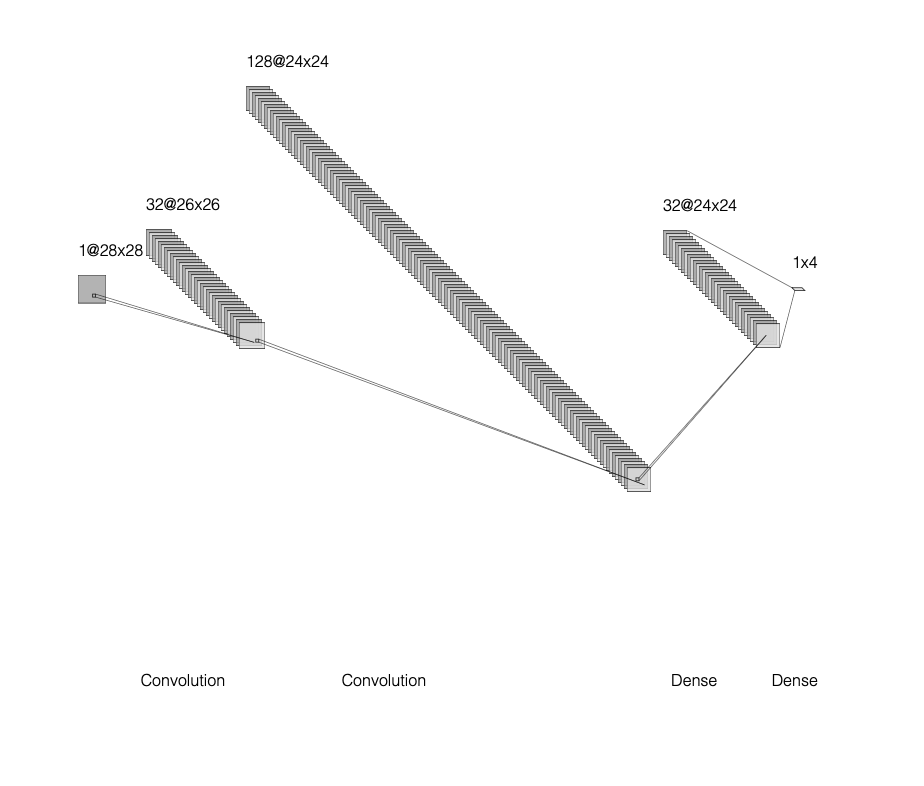
\includegraphics[width=0.9\linewidth]{training_model_structure.png}
    \caption{\small The structure of training model with 4 layers}
    \label{fig:training_model_structure}
\end{figure}

To find the relation between the training model complexity and the universal perturbation, the dataset complexity level(number of layers in images generator) should be fixed on 4.

\subsection{Generating the universal perturbation}

Some hyper-parameters setting
\begin{itemize}
    \item Images used to train the universal perturbation: 400 and 100 for each class
    \item Baseline Method to generate perturbation: Deep Fool
    \item Fooling rate $> 70\%$
    \item Metric to calculate the magnitude of universal perturbation: Infinity Norm $||\xi||_\infty$
    \item Maximum number of iterations to train the universal perturbation: 10
\end{itemize}

\section{Result Analysis}

\begin{table}
\begin{center}
\begin{tabular}{ |c|c|c| } 
\hline
Data complexity & Model layers & $\xi$ \\
\hline
0 & & 4.2 \\ 
1 & & 2.0 \\ 
2 & & 1.8 \\
3 & & 1.8 \\ 
4 & & 1.8 \\ 
5 & \multirow{4} & 1.6 \\ 
6 & & 1.6 \\ 
7 & & 1.6 \\ 
8 & & 1.1 \\ 
9 & & 0.9 \\ 
\hline
\end{tabular}
\end{center}
\caption{Relation between dataset complexity and universal perturbation}
\label{table:dc_up_table}
\end{table}

\begin{figure}[h]
    \centering
    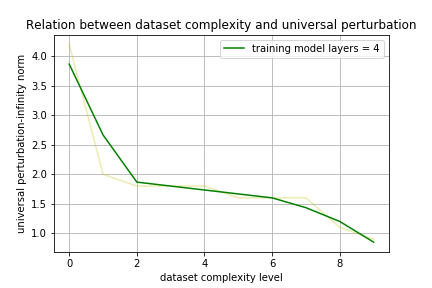
\includegraphics[width=1\linewidth]{dc_up.png}
    \caption{\small Relation between dataset complexity and universal perturbation}
    \label{fig:dc_up}
\end{figure}

To visualize the Table \ref{table:dc_up_table}, see Figure~ \ref{fig:dc_up}. The shallow line represents the original data points and solid line is the more smooth line generated from the shallow one by using Savitzky-Golay filter~\cite{LUO20051429}. As shown in table, for example, when the data complexity is 0 and the number of training models layers is 4, if adding the universal perturbation is smaller than 4.2, then the fooling rate will less than $70\%$. The value of $\xi$ is the boundary to determine whether fooling rate is greater or smaller than $70\%$. So this value can show how easy the universal perturbation exists.

See Figure~ \ref{fig:per2}, when dataset complexity level is 1, adding universal perturbation with infinity norm 2.0 can fool training model to recognise one image of class 2 as class 3.
\begin{figure}[h]
    \centering
    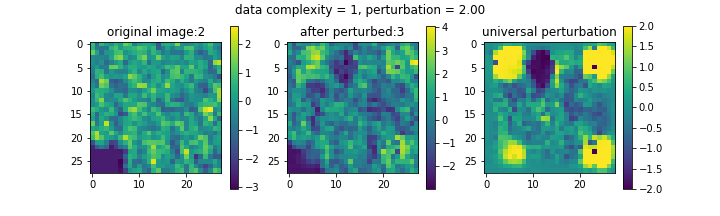
\includegraphics[width=1\linewidth]{model-c1-l4-pb-per2.png}
    \caption{\small Example of universal perturbation with infinity norm 2.0}
    \label{fig:per2}
\end{figure}

See Figure~ \ref{fig:per09}, when dataset complexity level is 9, adding universal perturbation with infinity norm 0.9 can fool training model to recognise one image of class 1 as class 3.
\begin{figure}[h]
    \centering
    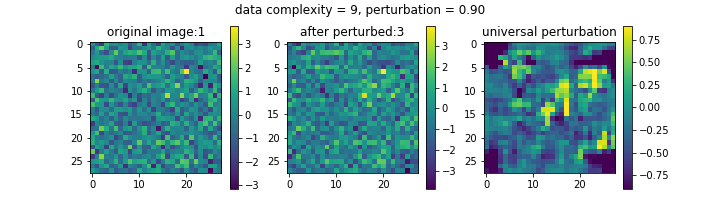
\includegraphics[width=1\linewidth]{model-c9-l4-pb-per09.png}
    \caption{\small Example of universal perturbation with infinity norm 0.9}
    \label{fig:per09}
\end{figure}

To compare these two universal perturbations, the universal perturbation with larger infinity norm changed the original images information more, like brute force  to change one class image to another class. This kind of universal perturbation is relatively meaningless than slight perturbation in real world.

When the dataset become more complex, smaller universal perturbation can be added on images to fool the training model well.

\begin{table}
\begin{center}
\begin{tabular}{ |c|c|c| } 
\hline
Model layers & Data Complexity & $\xi$ \\
\hline
3 & & 2.7 \\ 
5 & & 2.4 \\ 
8 & & 1.5 \\
11 & \multirow{4} & 1.5 \\ 
14 & & 1.3 \\ 
17 & & 1.2 \\ 
20 & & 1.5 \\ 
\hline
\end{tabular}
\end{center}
\caption{Relation between training model complexity and universal perturbation}
\label{table:tmc_up_table}
\end{table}

To visualize the Table \ref{table:tmc_up_table}, see Figure~ \ref{fig:tmc_up}.
\begin{figure}[h]
    \centering
    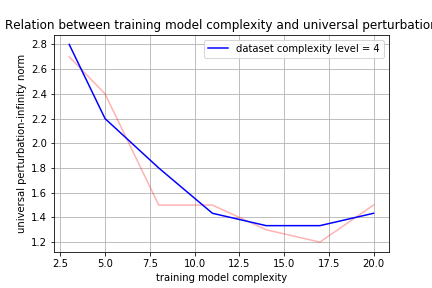
\includegraphics[width=1\linewidth]{tmc_up.png}
    \caption{\small Relation between training model complexity and universal perturbation}
    \label{fig:tmc_up}
\end{figure}

Overall, when the training model become more complex, smaller universal perturbation can be added on images to fool the training model well. In this experiment, the universal perturbation generated from 20 layers training model is slightly larger than those generated from 14 and 17 layers training models. This is probably because some bias of this experiment occur.

\section{Discussion and Future Work}
\subsection{An explanation to universal perturbation}
In ~\cite{Moosavi-Dezfooli_2017_CVPR}, Moosavi-Dezfooli presented an explanation to the vulnerability of DNN classifiers to universal perturbation. Moosavi-Dezfooli compared Universal Perturbation with 1) random noise 2)adversarial perturbation computed by single sample 3)mean of images (images bias) 4)sum of adversarial perturbation over $X$, and the result shows that Universal Perturbation can obtain the highest fooling rate with small $\xi$(see Figure~\ref{fig:MD_UAP1}).

The result shows that by calculating DeepFool perturbation over all data points, universal perturbation must capture some of the common characteristics of the decision boundary, in other word, there is geometric redundancy in the decision boundary (different data points’ direction to its nearest decision boundary is correlated), and the algorithm learned from the data about such a correlation. 
By calculating DeepFool perturbation, we are actually finding a normal vector of a data point to its nearest decision boundary. To quantify the linear correlation the structure of decision boundaries (to what extent there is a common direction vector which most data points share), Moosavi-Dezfooli calculated each data point’s normal vector to its respective nearest decision boundary for data points in the validation set:
 \begin{figure}
    \centering
    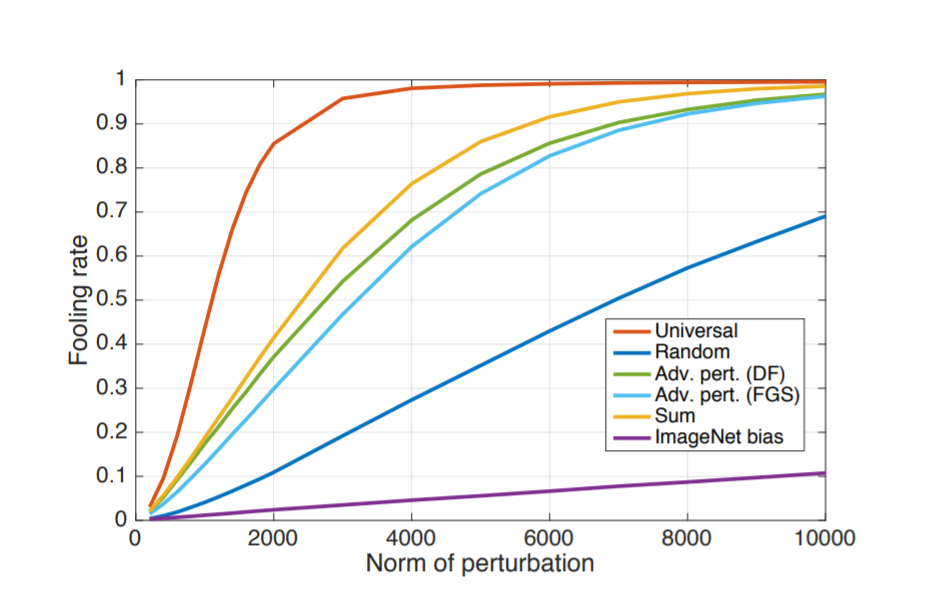
\includegraphics[width=\linewidth]{MD_UAP1.png}
    \caption{\small  Comparison between fooling rates of different perturbations. Experiments performed on the CaffeNet architecture. \cite{Moosavi-Dezfooli_2017_CVPR}}
    \label{fig:MD_UAP1}
\end{figure}
\begin{equation*}
N=\left[\frac{r\left(x_{1}\right)}{\left\|r\left(x_{1}\right)\right\|_{2}} \ldots \frac{r\left(x_{n}\right)}{\left\|r\left(x_{n}\right)\right\|_{2}}\right]
\end{equation*}
Moosavi-Dezfooli calculated the singular values of matrix N and compare it with the singular values computed from uniformly sampled random noise matrix of the same shape(see Figure~\ref{fig:MD_UAP2}). 
 \begin{figure}
    \centering
    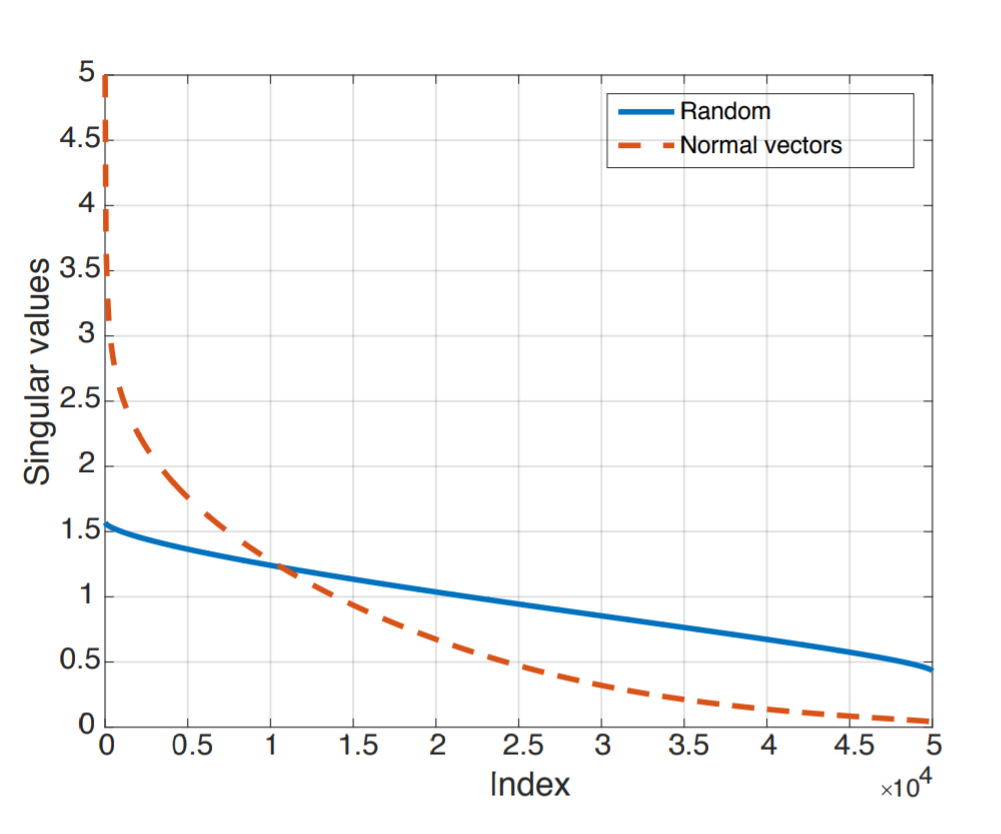
\includegraphics[width=\linewidth]{MD_UAP2.png}
    \caption{\small Singular values of matrix \tettit{$N$} containing normal vectors to the decision boundary \cite{Moosavi-Dezfooli_2017_CVPR}}
    \label{fig:MD_UAP2}
\end{figure}

The singular values of N decay quickly, while the random noise’s singular values decay gently, which indicate that there exists linear redundancy in the decision boundary. In other word, there exists lower dimensional vector space $\mathcal{S}$ which contains most normal vectors of natural images in ImageNet to their nearest decision boundary. As a result, the existence of universal perturbation may due to the subspace that contains most normal vectors to the decision boundary. Actually, random vector that belong to a subspace that spanned by the first 100 singular vectors of N can fool near 38\% natural images in ImageNet, significantly better than random noise, which is 10\%.
\subsection{Future works}
For the bias in the experiment, more experiments should be done to analyse why this noise happen. For example, adding more than 20 layers in training model to analyze the infinity norm of the universal perturbation.

In this experiment, adding more convolutional layers in images generator can control the complexity level of the datasets. But in real world, some methods should be found or applied to evaluate semantic datasets complexity, such as spectral metric~\cite{Branchaud-Charron_2019_CVPR} or other complexity measures.

Calculate the difference of different class images in various complexity level datasets by using Kullback–Leibler divergence of other metrics. Find whether the difference of different class images in complex datasets is smaller than that in simple datasets. 

Test the universality of universal perturbation and find whether there is a "global" universal perturbation. In this experiment, universal perturbation is "locally" universal, meaning it is a pattern can fool the training model trained on a certain dataset and may not fool the training model trained on other datasets in a high fooling rate.


\section{Conclusion}
To summarise, when the dataset and training model become more and more complex, the decision boundary gradually become unclear and difficult to be learnt by classifiers. So, there may exist an universal perturbation or a pattern to disturb original dataset information, inducing one class images can be added a small perturbation to "skip" into other decision areas.

% \textbf{Do not} include acknowledgements in the initial version of
% the paper submitted for blind review.

% If a paper is accepted, the final camera-ready version can (and
% probably should) include acknowledgements. In this case, please
% place such acknowledgements in an unnumbered section at the
% end of the paper. Typically, this will include thanks to reviewers
% who gave useful comments, to colleagues who contributed to the ideas,
% and to funding agencies and corporate sponsors that provided financial
% support.


% In the unusual situation where you want a paper to appear in the
% references without citing it in the main text, use \nocite
\nocite{*}

\bibliography{reference}
\bibliographystyle{icml2019}


\end{document}